\documentclass[10pt]{article}
\usepackage[utf8]{inputenc}
\usepackage{amsmath}
\usepackage{epsfig}
\usepackage{enumerate}
\usepackage{float}
\usepackage{listings}
\frenchspacing
\linespread{1.2}                                          %espacio entre líneas
\setlength{\parskip}{1.5ex plus 0.2ex minus 0.2ex}        %espacio entre párrafos
\setlength{\columnsep}{0.9cm}  				  %espacio entre columnas
\usepackage{indentfirst}
\usepackage{graphicx}
\usepackage{verbatim}
\usepackage{url}
\usepackage{multicol}
\usepackage{geometry}
\usepackage{fancyhdr}
\usepackage{moreverb}

\geometry{tmargin=4.5cm, lmargin=3.0cm, rmargin=2.5cm, bmargin=2.0cm}

\newcommand\R{R} %Sentencia para crear nuevos comandos.
\newenvironment{keywords}{\begin{description}\item[Keywords:]}{\end{description}}

\title{
\center{
	\textbf{Especificación de Requerimientos}
	}
\author{Author1 \\ \url{author1@csrg.inf.utfsm.cl} \\
	Author2 \\ \url{author2@csrg.inf.utfsm.cl} \\
	}
\date{Valparaíso, \today}
}

%\fancyhf{}
%\fancyhead[L]{Especificación de Requerimientos}
%\fancyhead[R]{\thepage}
%\fancyfoot[L]{{\small Desarrollo de una plataforma astroinformática para la administración y análisis inteligente de datos a gran escala}}
%\fancyfoot[R]{{\small }}
%\pagestyle{fancy}

\begin{document}
\maketitle

%\vspace{0.5cm}

%\begin{center}
%	\begin{abstract}
%		\input{include/abstract}
%	\end{abstract}
%\end{center}

%\vspace{0.4cm}

%\begin{center}
%\begin{keywords}
%Keyword1, keyword2.
%\end{keywords}
%\end{center}

%\vspace{1cm}

\thispagestyle{empty}

\newpage
\tableofcontents

\section{Resumen Ejecutivo}

\newpage
\section{Estado del Arte}

\newpage
\section{Requerimientos de ChiVO}

Los requerimientos se clasificarán en:
\begin{itemize}
	\item Necesidad: Esencial, deseable, opcional.
	\item Prioridad temporal: Alta, media, baja.
\end{itemize}

\begin{enumerate}
	\item \textbf{Buscar por coordenadas o región del cielo [Necesidad:
Esencial | Prioridad temporal: Alta]:}

Se podrán realizar búsquedas de posición mediante coordenadas y radio angular
(cónicas) o por región del cielo.

Los parámetros de las coordenadas pueden ser en distintos sistemas como
ecuatorial, eclíptico, galáctico o supergaláctico. Los parámetros ingresados se
convertirán al sistema de la fuente de datos, para así poder realizar las
búsquedas, IVOA utiliza los sistemas de coordenadas ICRS y ecuatoriales J2000.

En un principio, el sistema ofrecerá servicio de búsqueda por coordenadas
cónicas y más adelante, en caso de ser vía un portal web, se ofrecerá búsqueda
por región de cielo.

El sistema también deberá permitir buscar simultáneamente un listado de
coordenadas.

	\item \textbf{Buscar por nombre o tipo de objeto [Necesidad: Esencial |
Prioridad temporal: Alta]:}

El sistema deberá permitir buscar por nombres de objetos que se encuentren
definidos en Sesame, del Centre de Données astronomiques de Strasbourg (CDS).

Por otro lado, la búsqueda por tipo o subtipo de objeto, tales como estrellas
en formación, estrellas nebulosas planetarias, supernovas, galaxias, cometas,
entre otros, permitirá al usuario encontrar datos relacionados con una
problemática en especial. En un principio, el sistema realizará estas búsquedas
acorde a la información presente en los catálogos.

A futuro, el sistema deberá permitir minería de datos para detección de tipos
de objetos similares, esto es posible debido a que existen clasificaciones
discretas que permiten clasificar los objetos que se encuentran en las
observaciones.

Este tipo de búsquedas, se transforman en búsquedas por coordenadas, ya que al
buscar por un nombre, por ejemplo, Sesame responde con la correspondiente
ubicación del objeto en coordenadas. Y luego de ello se procede a realizar la
búsqueda por coordenadas correspondiente.

El resultado de la búsqueda deberá facilitar la obtención de datos para ser
analizados como secuencias de tiempo.

	\item \textbf{Buscar por metadatos espectrales (frecuencia y
resolución) [Necesidad: Esencial | Prioridad temporal: Alta]:}

Se podrán realizar búsquedas por metadatos espectrales, lo cual consiste en
búsqueda por banda o rango de frecuencia, búsquedas por líneas espectrales y
corrimiento al rojo o búsquedas por resolución espectral. Específicamente, hay
dos enfoques:
\begin{itemize}
	\item Galáctico: Por frecuencia en reposo y velocidad radial.
	\item Extragaláctico: Por frecuencia en reposo y corrimiento al rojo.
\end{itemize}

La Frecuencia en reposo incluye búsquedas por molécula, transición de molécula
(vibracional, rotacional o electrónica) o frecuencia de línea espectral.

	\item \textbf{Buscar por metadatos espaciales (resolución angular y
campos de visión) [Necesidad: Esencial | Prioridad temporal: Alta]:}

Se podrán realizar búsquedas espaciales en base a parámetros relacionados con
rangos de  resolución angular y campos de visión y siempre en base a
coordenadas.

Los parámetros de las coordenadas pueden ser en distintos sistemas como
ecuatorial, eclíptico, galáctico o supergaláctico. Los parámetros ingresados se
convertirán al sistema de la fuente de datos, para así poder realizar las
búsquedas.

Además, se podrá especificar parámetros relacionados con la forma de las
observaciones (rectangulares o redondas).

	\item \textbf{Buscar por metadatos temporales [Necesidad: Esencial | Prioridad temporal: Baja]:}
Se podrán realizar búsquedas por metadatos temporales que pueden ser
clasificadas en dos tipos de búsquedas: 
\begin{itemize} 
\item Cuando fue realizada la observación, incluyendo cuantas veces se observó
un objeto y/o el intervalo entre observaciones.  
\item Nivel de ruido, duración de la observación o tiempo de integración. Dado
un ruido, se necesita un tiempo de integración que depende de la frecuencia
observada y del clima.  
\end{itemize}

	\item \textbf{Buscar por polarización [Necesidad: Esencial | Prioridad
temporal: Media]:}

Cada imagen se puede dividir en cuatro parámetros llamados los parámetros de
Stokes o en dos: izquierda y derecha. En radio astronomía no suele hacerse
debido a que requiere una alta precisión del instrumento, en el caso de ALMA se
requiere que esté lista la calibración.

El sistema debe permitir buscar si existe o no polarización en alguno de los
parámetros de Stokes: I, Q, U o V.

	\item \textbf{Cruzamiento de información [Necesidad: Esencial |
Prioridad temporal: Alta]:}

La búsqueda cruzada debe permitir al usuario realizar las búsquedas mencionadas
anteriormente en múltiples fuentes de datos distribuidos globalmente, sin
importar su tipo. Lo que permitirá obtener todos los datos existentes sobre un
objeto o área espacial y así evitar realizar observaciones innecesarias debido
al descubrimiento de observaciones existentes. Los tipos de fuentes pueden ser
Sesame, ALMA u Observatorios Virtuales, que cumplan con los estándares de IVOA.

La búsqueda de un mismo objeto en distintas fuentes de información, debido a
que en cada fuente el instrumento tiene un margen de error en cuanto a la
posición del objeto, debe ser capaz de realizar una intersección entre los
radios de margen de error de las distintas fuentes para identificar al objeto
en una búsqueda cruzada.

	\item \textbf{Simulaciones [Necesidad: Deseable | Prioridad temporal:
Baja]:}

Es a veces necesario realizar comparaciones con observaciones obtenidas a
través de simulaciones, así cómo es costoso  realizar una observación dos
veces, para una simulación puede ser aún más, debido a que dependiendo de la
magnitud, hay simulaciones que requieren una gran capacidad de cómputo.

	\item \textbf{Servicios Bibliográficos [Necesidad: Deseable | Prioridad
temporal: Baja]:}

Las herramientas existentes cumplen su función correctamente. Por ello, basta
con que al buscar un objeto, se desplieguen también resultados de
investigaciones que se hayan realizado al respecto con un enlace a SIMBAD o
similares.

\end{enumerate}

\newpage
\section{Capa de modelo de datos}
\subsection{Estándares y Protocolos IVOA}
Breve descripción de los protocolos y estándares a considerar. Es recomendado
el estudio de éstos en el siguiente orden:

\begin{enumerate}
	\item[a.] \textbf{Observation Core Data Model}: Define los componentes
principales de todos los metadatos accesibles que tienen un rol en el
descubrimiento de las observaciones.  Requerimientos: Todos, debido a que es el
Modelo de Datos base. \url{http://www.ivoa.net/documents/ObsCore/index.html} 

	\item[b.] \textbf{Units}: Define las prácticas comunes en la
manipulación de unidades en los metadatos astronómicos y define una
representación consistente en los servicios dentro de un Observatorio Virtual.
Necesario para: Observation Core Data Model, Simple Spectral Line Data Model,
Characterisation Data Model, Simulations Data Model.
\url{http://www.ivoa.net/documents/VOUnits/index.html}

	\item[c.] \textbf{Utypes}: Relacionado con Units, Utypes son nombres
que definen inequívocamente los elementos de los metadatos. Necesario para:
Observation Core Data Model, Simple Spectral Line Data Model, Characterisation
Data Model, Simulations Data Model.
\url{http://www.ivoa.net/documents/Notes/UTypesUsage/index.html}

	\item[d.] \textbf{Simple Spectral Line Data Model}: Describe las
transiciones de líneas espectrales. Podría ser necesario, de otra manera, la
información puede estar contenida en el Observation Core Data Model.
Requerimientos: (3) Buscar por metadatos espectrales (frecuencia y resolución).
\url{http://www.ivoa.net/documents/SSLDM/}

	\item[e.] Characterisation Data Model: Define y organiza todos los
metadatos necesarios para describir cómo un conjunto de datos ocupa un espacio
físico multidimensional, cuantitativamente y, cuando es relevante,
cualitativamente. Requerimientos: (3) Buscar por metadatos espectrales
(frecuencia y resolución), (4) Buscar por metadatos espaciales (resolución
angular y campos de visión).
\url{http://www.ivoa.net/Documents/latest/ImplementationCharacterisation.html}

	\item Space Time Coordinate metadata: Describe metadatos espaciales y
temporales. Podría ser necesario para usos específicos de tiempo-espacio.
Requerimientos: (1) Buscar por coordenadas o región del cielo, (2) Buscar por
nombre o  tipo de objeto, (4) Buscar por metadatos espaciales (resolución
angular y campos de visión), (5) Buscar por metadatos temporales.
\url{http://www.ivoa.net/Documents/latest/STC-Model.html}

	\item Simulations Data Model: Define y organiza todos los metadatos
necesarios para describir conjuntos de datos de simulaciones. Requerimientos:
(7) Simulaciones. \url{http://www.ivoa.net/documents/SimDM/index.html}
\end{enumerate}

\subsection{Modelo de datos}

Se especificará una tabla con los atributos y la descripción de cada uno, en
concordancia a los recomendado con IVOA.

\begin{table}[h!t]
	\centering
	\begin{tabular}{|l|l|l|} 
		\hline
		Nombre de la columna & Unidad & Descripción \\
		\hline
		dataproduct\_type & sin unidad & Tipo de dato lógico \\
		calib\_level & sin unidad & Nivel de calibración \\
		obs\_collection & sin unidad & Nombre de la colección de datos \\
		obs\_id & sin unidad & ID de observación \\
		obs\_publisher\_id & sin unidad & Identificador de datos entregado por el publisher \\
		access\_url & sin unidad & URL para acceder a los datos \\
		access\_format & sin unidad & Formato del archivo \\
		access\_estsize & kbyte & Tamaño estimado en KB \\
		target\_name & sin unidad & Objeto astronómico observado \\
		s\_ra & grados & RA central \\
		s\_dec & grados & Dec central \\
		s\_fov & grados & Diámetros de la región cubierta \\
		s\_region & sin unidad & Región cubierta en ADQL \\
		s\_resolution & arco segundos & Resolución espacial \\
		t\_min & días & Hora de comienzo \\
		t\_max & días & Hora de fin \\
		t\_exptime & segundos & Tiempo de exposición \\
		t\_resolution & segundos & Resolución temporal \\
		em\_min & minutos & Comienzo en coordenadas espectrales \\
		em\_max & minutos & Fin en coordenadas espectrales \\
		em\_res\_power & sin unidad & Poder de resolución espectral \\
		o\_ucd & sin unidad & UCD observable \\
		pol\_states & sin unidad & Lista de estados de polarización \\
		facility\_name & sin unidad & Nombre del lugar usado para la observación \\
		instrument\_name & sin unidad & Nombre del instrumento usado para la observación \\
		\hline
	\end{tabular}
	\caption{Integrantes de IVOA}
	\label{table:tap_column_name}
\end{table}


\newpage
\section{Capa de aplicación}


La definición de requerimientos de datos involucra en particular a una área de
arquitectura de software recomendada por IVOA. Esta capa es la de
estándares y protocolos de acceso a los datos (Data Access Protocol Standards).

Los datos y metadatos astronómicos están siendo distribuidos mediante distintos
mecanismos que le permitan a la comunidad astronómica y científica acceder a
ellos de forma fácil y estandarizada. Por lo general estos accesos son mediante
páginas web, aplicaciones de escritorio, servicios File Transfer Protocol
(FTP), etc. La colaboración de distintos observatorios virtuales ha permitido
crear protocolos estandarizados para consultar y acceder datos y metadatos de
distintas fuentes de información. Estos protocolos fueron creados para permitir
que la implementación fuese más fácil.

Durante la ejecución del proyecto se han estudiado estos protocolos, enmarcado
en la idea de observatorio virtual, y la arquitectura que se debe respetar.

\textbf{Estándares y Protocolos de acceso de datos} \begin{enumerate} \item
\textbf{Buscar por coordenadas o región del cielo}: las búsquedas por
coordenadas en el espacio, involucra la definición de una coordenada RA/DEC, y
además de un radio angular. Este tipo de consultas están consideradas dentro de
un protocolo de acceso de datos definido por IVOA, el cual se llama Simple Cone
Search.  Otra búsqueda puede ser por región del cielo definiendo una región
rectangular, el protocolo relacionado es Simple Image Access Protocol.

	\item \textbf{Buscar por metadatos espaciales}: las búsquedas
espaciales requieren definir parámetros de rangos de resolución angular y
campos de visión en base a coordenadas. El protocolo de acceso con el cual se
deberá implementar este requerimiento es mediante Table Access Protocol,
basándose en Astronomical Data Query Language.

	\item \textbf{Buscar por nombre o tipo de objeto}: este requerimiento
considera buscar en ciertos catálogos astronómicos los cuales se definirán a lo
largo del proyecto, teniendo en consideración qué tipo de datos necesitará la
comunidad astronómica y los participantes de este proyecto. Los catálogos
astronómicos son objetos astronómicos agrupados por características en común.
Para este punto se tendrá que estudiar y aprovechar el marco de trabajo que
provee IVOA en su grupo de Semánticas.

	\item \textbf{Buscar por metadatos espectrales}: las búsquedas por
metadatos espectrales se basará en búsqueda por banda o rango de frecuencia,
líneas espectrales, búsquedas por resolución espectral y redshift. Este tipo de
búsqueda se realizará mediante el uso de los protocolos Table Access Protocol y
Simple Spectra Acess Protocol.

	\item \textbf{Buscar por metadatos temporales}: la búsqueda por
metadatos temporales se enfocará a fechas de cuando se hizo cierta observación,
duración, veces que se observó, etc. Esto se cubrirá usando Table Access
Protocol.

	\item \textbf{Cruzamiento de información}: este punto está relacionado
al punto 3. Lo que se busca es poder brindarle a la comunidad astronómica
distintas fuentes de datos, aparte de los datos de ALMA. Para ello se definirán
a lo largo del proyecto, cuales son los de interés, qué catálogos y de qué
observatorios virtuales se obtendrán. Cabe destacar que estos procesos son
estándares ya que todos los servicios están normados por los mismos protocolos.

	\item \textbf{Simulaciones}: se buscará sobre servicios que posean
datos de simulaciones para permitir comparaciones teóricas con reales. En IVOA
el protocolo relacionado a Simulations Data Access Layer, está aún en
desarrollo, sin embargo hay versiones iniciales del estándar.

	\item \textbf{Servicios Bibliográficos}: durante la ejecución del
proyecto, y después cuando ChiVO esté en funcionamiento, existirán fuentes de
documentación científica, ya sean reportes técnicos o papers. Se implementará
un buscador que a partir de información como: rango de año, autor, fuente en
estudio, se le entregue al usuario una lista de artículos que hayan calzado con
la búsqueda.  Algo similar a como funciona SIMBAD.

	\item \textbf{Herramientas de análisis}: durante la ejecución del
proyecto se implementarán herramientas de análisis de datos de gran escala, las
cuales serán integradas dentro de lo posible (si es que se pueden usar de forma
web) a la plataforma online, en otro caso, se proveerá acceso y documentación
de como usar cada herramienta, tutoriales y casos de ejemplo.
\end{enumerate}

\newpage
\section{Capa Vista Controlador}

Las propuestas iniciales (maquetas) están siendo probadas en
\href{http://chivoalpha.herokuapp.com/query}{Link Query Form}. Esta capa de
está desarrollada en base a los requerimientos funcionales del sistema, los
cuales plantean un sistema que sea fácil de acceder y de manejar. Para ello se
piensa inicialmente desarrollar una forma de consulta básica y avanzada. 

En adelante se presentan las actuales snapshots de la
maqueta.

\begin{figure}[h!t]
         \begin{center}
                 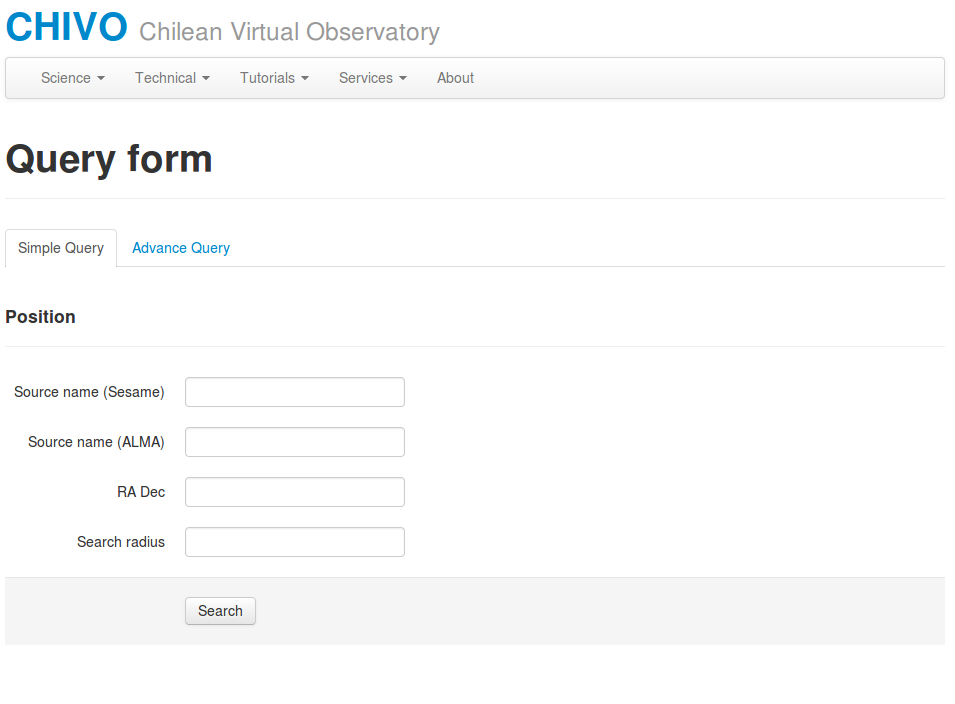
\includegraphics[width=0.8\textheight]{img/snap1.png}
                 \caption{Basic Query Form}
         \end{center}
\end{figure}

\newpage

\begin{figure}[h!t]
         \begin{center}
                 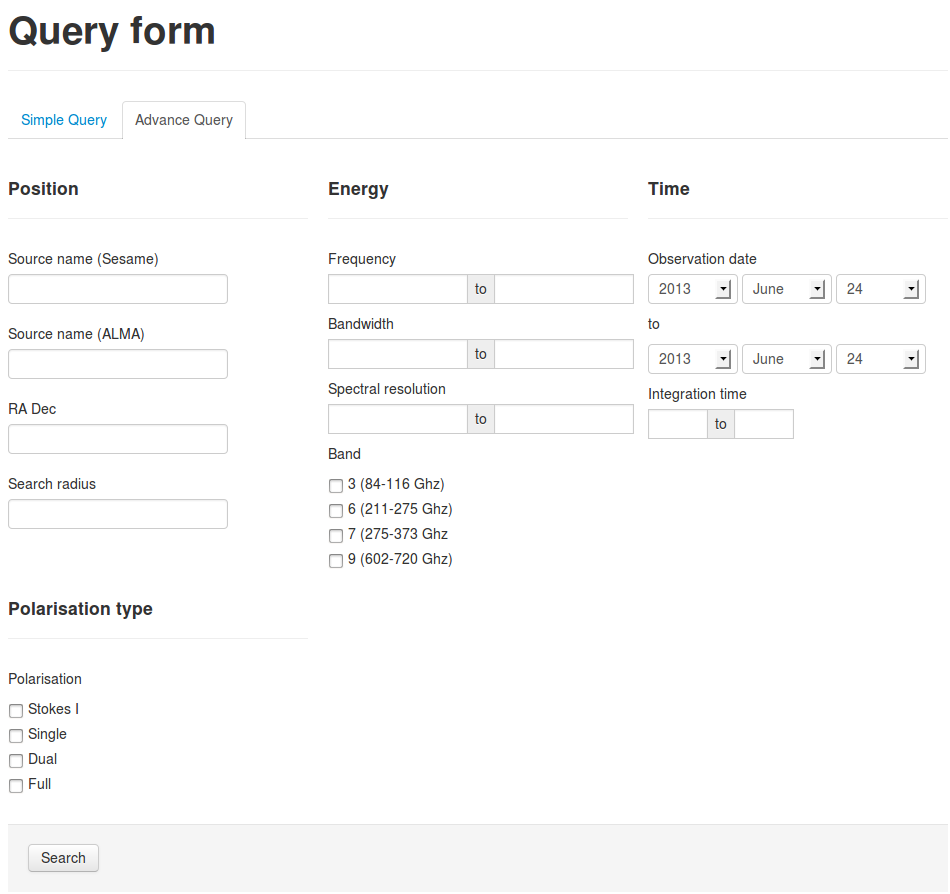
\includegraphics[width=0.8\textheight]{img/snap2.png}
                 \caption{Advanced Query Form}
         \end{center}
\end{figure}

\newpage

\begin{figure}[h!t]
         \begin{center}
                 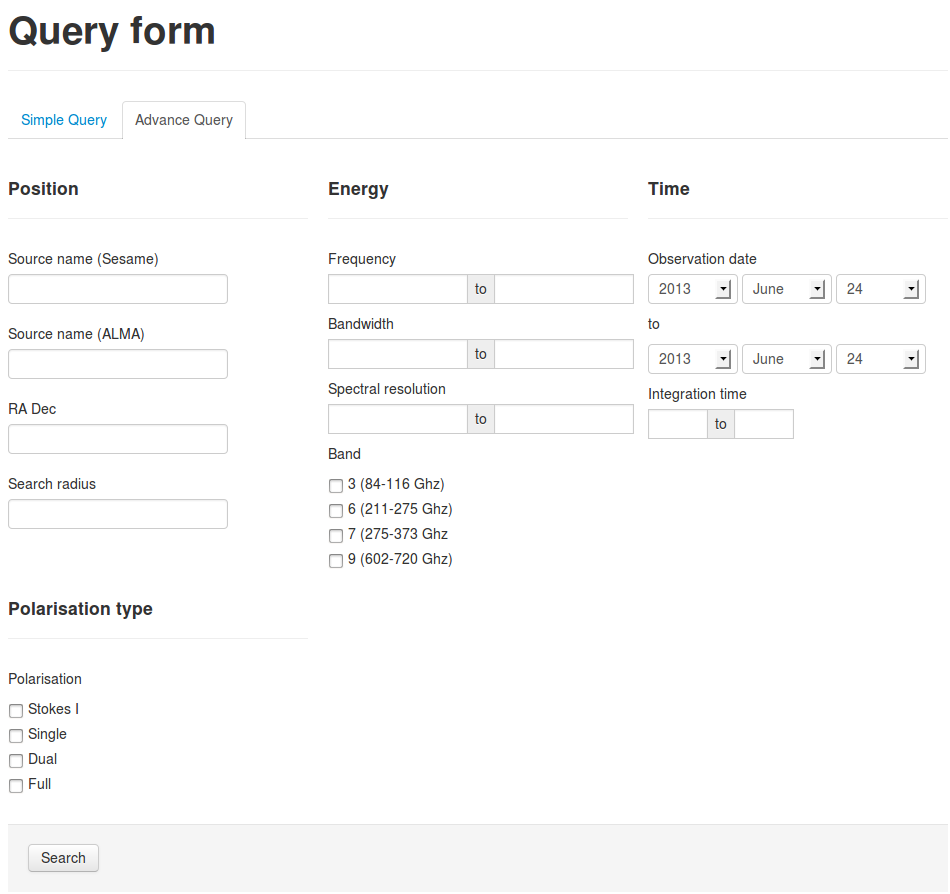
\includegraphics[width=0.8\textheight]{img/snap2.png}
                 \caption{Results}
         \end{center}
\end{figure}

\newpage
\section{Anexos}
\subsection{IVOA Architecture}
El VO's es un framework que ayuda a resolver distintos
problemas que enfrenta la comunidad astronómica a lo largo del mundo.  Uno de
los problemas está relacionado al acceso a los datos, por lo que en IVOA
diseñaron tecnologías y estándares formalmente definidos, que permitan el de
acceso unificado y transparente a distintos servidores con datos astronómicos.

El beneficio que conlleva es considerable, ya que estos
estándares, protocolos, tecnologías y arquitectura, ayudan a la comunidad al
proceso de creación de servicios, portales web, aplicaciones de escritorio,
etc. Todo visto del punto de vista de ingeniería de software.

\subsubsection{Arquitectura VO por Nivel}

IVOA dentro de sus documentos presenta distintos niveles de arquitectura
\cite{ivoa_arch}, con el objetivo de ir aclarando incrementalmente las
funcionalidades (basadas en necesidades) que requiere un VO.

\textbf{Arquitectura Nivel 0} %~\ref{fig:nivel0}\\


La arquitectura más básica que aclara el concepto de VO, se compone por 3
capas:

\begin{enumerate}
    \item Capa de recursos:
          compilado de datos astronómicos provenientes de distintos instrumentos.
    \item Capa de usuarios:
          investigadores que buscan consumir datos.
    \item Capa intermedia:
          es la capa que permite conectar las dos
          capas anteriores de manera transparente para los investigadores.
          Esta interacción se puede llevar a cabo buscando u obteniendo datos.
\end{enumerate}

%\begin{figure*}[h!t]
\begin{figure*}
    \centering
    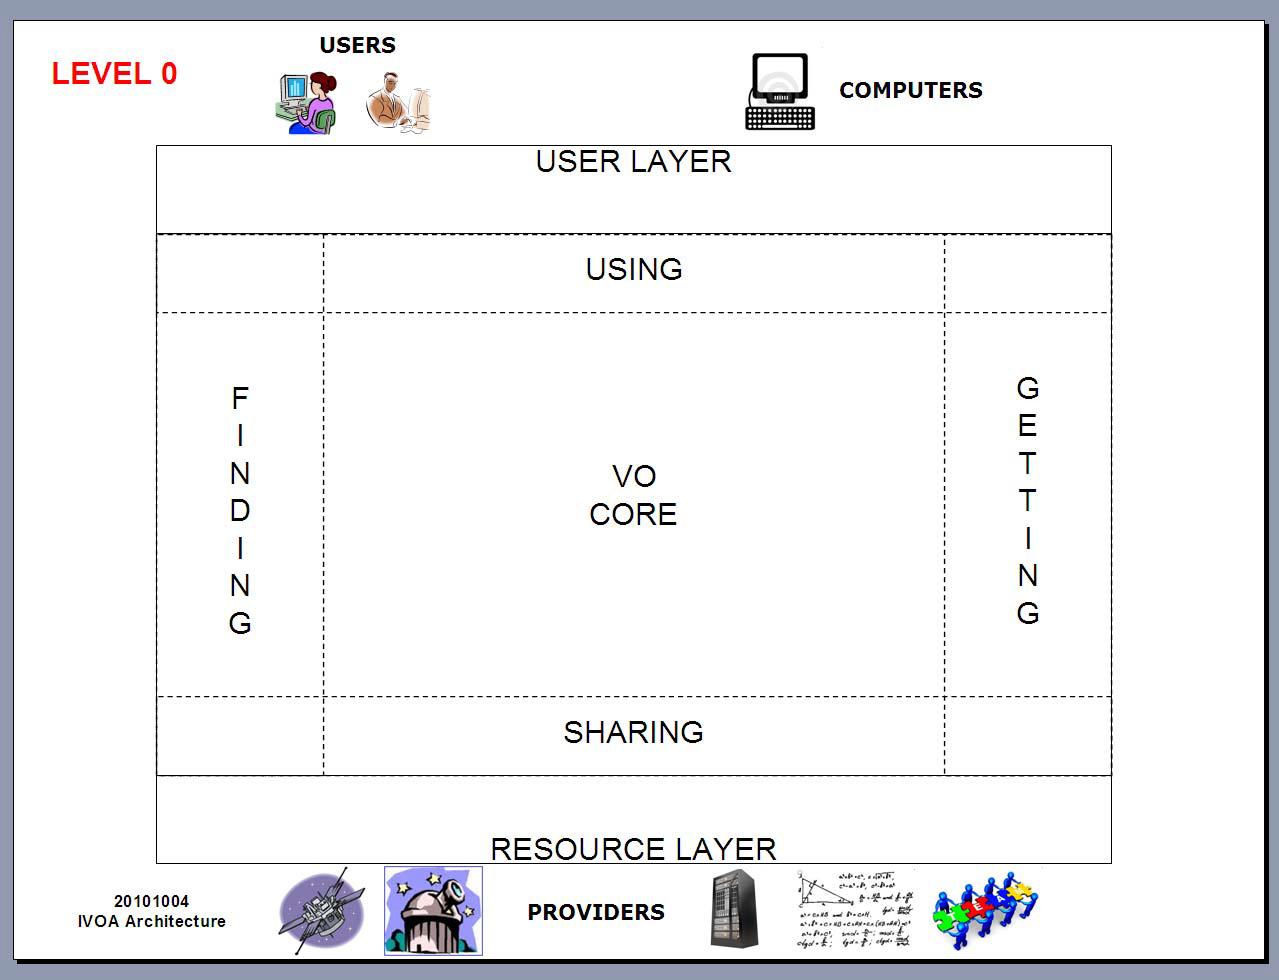
\includegraphics[width=0.7\textwidth]{img/arquitectura_0.png}
    \caption{Arquitectura Nivel 0}
    \label{fig:nivel0}
\end{figure*}

\textbf{Arquitectura Nivel 1}%~\ref{fig:nivel1}


La arquitectura nivel 1 mantiene la misma cantidad de capa pero se especifica:
\begin{enumerate}
    \item Capa de recursos:
          está compuesto de colección de datos y provenientes de distintos
          servidores.
    \item Capa de usuarios:
          un consumidor puede querer acceder a los datos desde un navegador,
          escritorio, o mediante un script.
    \item Capa intermedia:
          crea un framework para compartir los datos, compuesto por VOQL,
          Data Models, Semantics, Formats.
\end{enumerate}

%\begin{figure*}[h!t]
\begin{figure*}
    \centering
    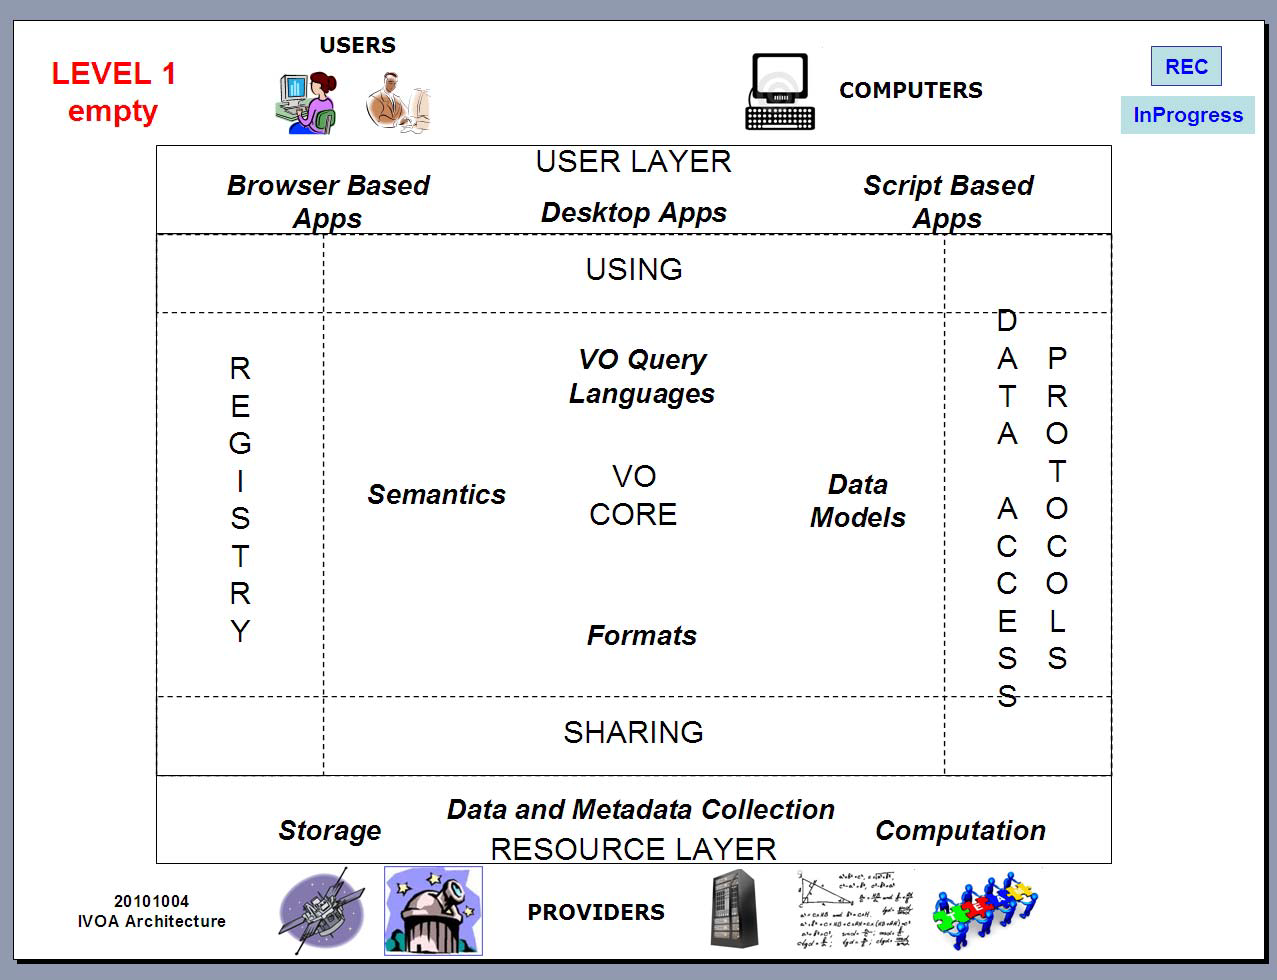
\includegraphics[width=0.7\textwidth]{img/arquitectura_1.png}
    \caption{Arquitectura Nivel 1}
    \label{fig:nivel1}
\end{figure*}

\textbf{Arquitectura Nivel 2}%~\ref{fig:nivel2}


La arquitectura nivel 2 es lo que se entiende por un VO regido por estándares
y protocoloes de IVOA.
La idea de esta figura es seccionar cada estándar relacionándolo específicamente
a la capa a la cual pertenece.

%\begin{figure*}[h!t]
\begin{figure*}
    \centering
    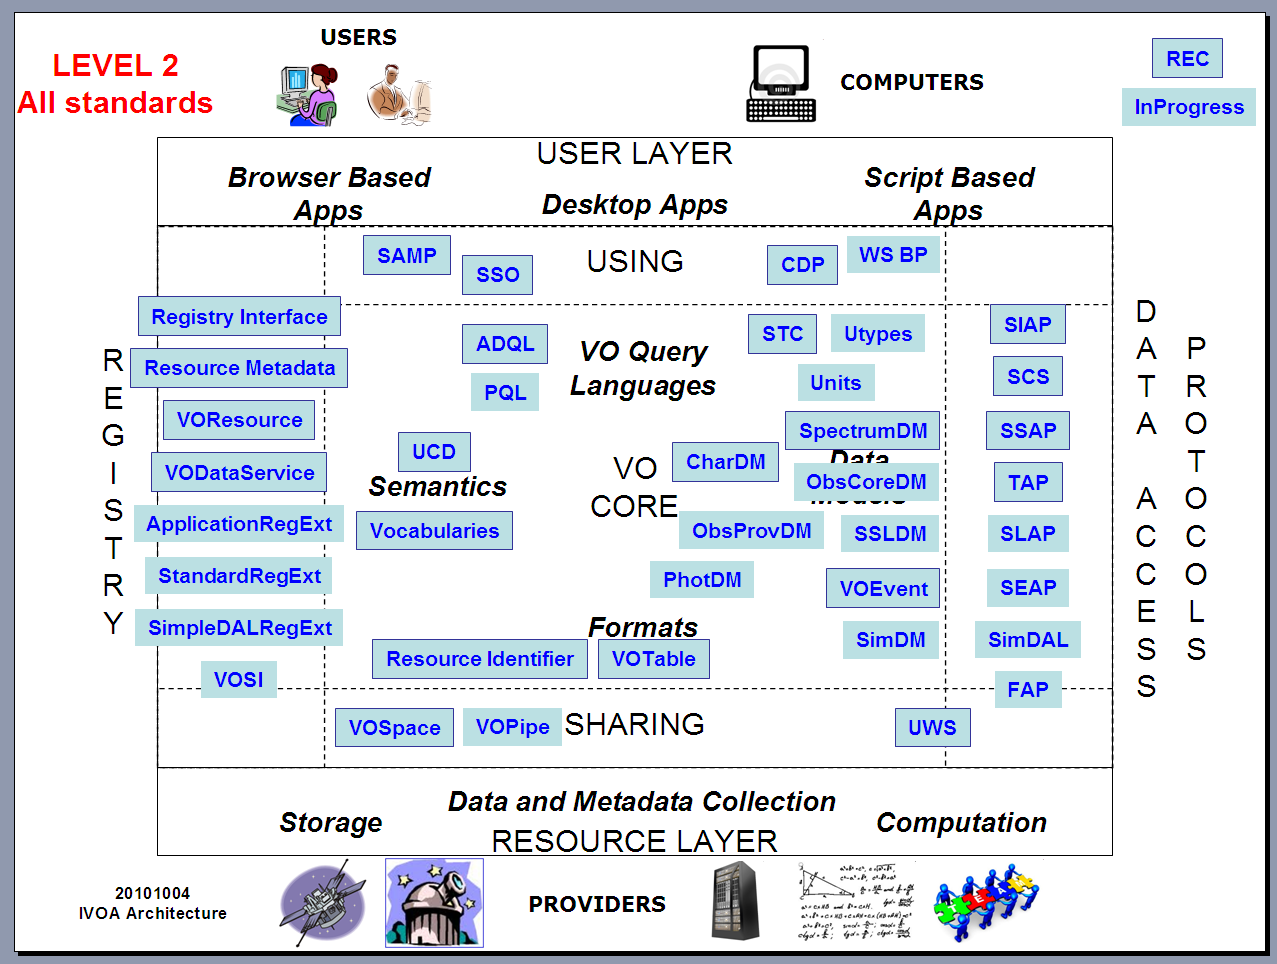
\includegraphics[width=0.7\textwidth]{img/arquitectura_2.png}
    \caption{Arquitectura Nivel 2}
    \label{fig:nivel2}
\end{figure*}


\subsection{Simple Cone Search Protocol}
\subsection{Simple Image Access Protocol}
\subsection{Astronomical Data Query Language}
\subsection{Semantics}
\subsection{Simple Spectra Access Protocol}
\subsection{SIMBAD}


\newpage
\thispagestyle{empty}
\addcontentsline{toc}{section}{Bibliography}

%\nocite{*}
%\bibliographystyle{alpha}
%\bibliography{report}

\end{document}
